\hypertarget{weebles}{%
\section{Weebles}\label{weebles}}

\begin{figure}[!ht]
  \begin{adjustwidth}{-\oddsidemargin-1in}{-\rightmargin}
    \centering
    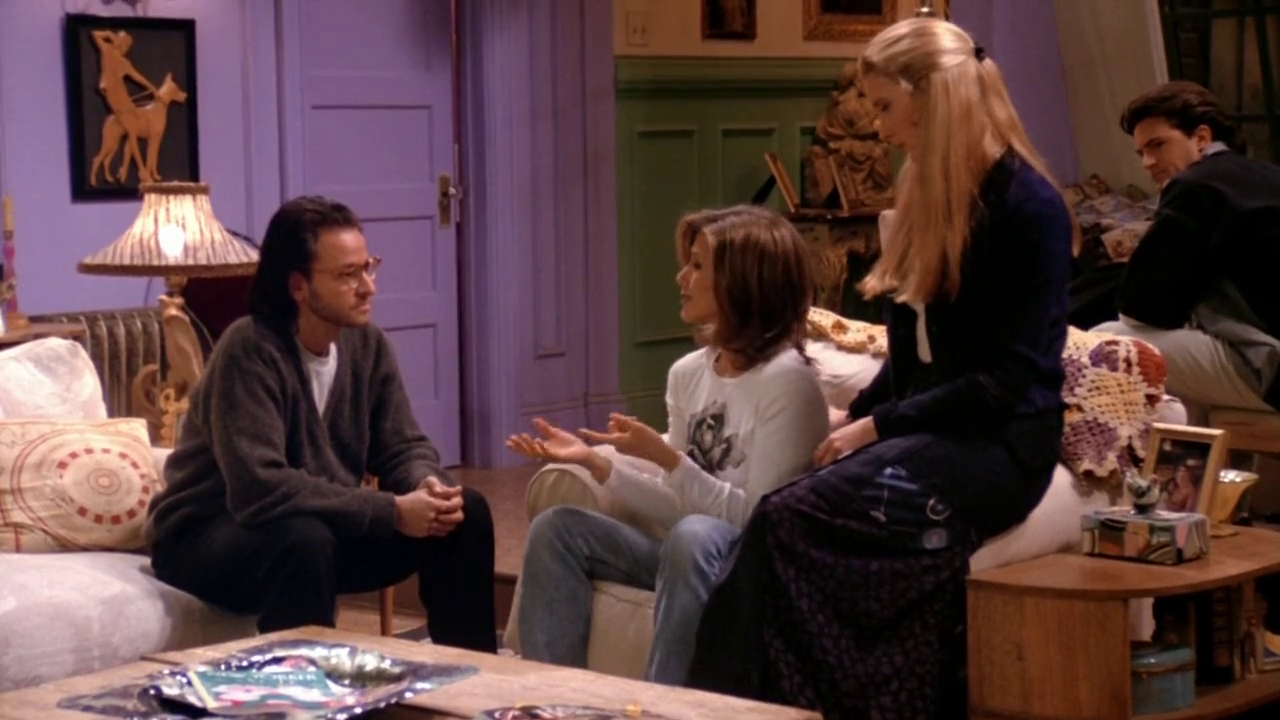
\includegraphics[trim={0 10cm 0 1cm,}, clip, width=\paperwidth]{./S01/img/13/weebles.png}
    % \caption{Weebles\label{fig:weebles}}
  \end{adjustwidth}
\end{figure}

\begin{tcolorbox}[enhanced,center upper,
    drop fuzzy shadow southeast, boxrule=0.3pt,
    lower separated=false, breakable,
    colframe=black!30!dialogoBorder,colback=white]
\begin{minipage}[c]{0.16\linewidth}
  \raisebox{\dimexpr-\height+\ht\strutbox\relax}{
    \centering 
\includegraphics[width=1.4cm]{./assets/img/rachel.png}
  }
   & \centering \scriptsize{Rachel}
\end{minipage}
\hfill
\begin{minipage}[c]{0.8\linewidth}
  \textbf{- It wasn't just the Weebles, but it was the Weeble Play Palace, and the Weeble's Cruise Ship, which had this little lifeboat for the Weebles to wobble in.}\\
  - Não foram só os Weebles, foi o palácio dos Weebles, e o navio dos Weebles, com barquinhos salva-vidas para não se afogarem.
\end{minipage}
\end{tcolorbox}

Abrindo seu coração para o Roger \emph{(I hate that guy!)} sobre sua
infância, Rachel menciona \emph{Weebles} (1971), um brinquedo em formato
de ovo com um peso na parte de baixo que o fazia ficar em pé. Daí o
bordão \textbf{Weebles wobble, but they don't fall down}, que em
português é algo como \textbf{Weebles balançam, mas não
caem}.\footnote{\sloppy Weebles - Wikipédia. \url{https://en.wikipedia.org/wiki/Weeble}}

\begin{figure}
  \centering
  \begin{tikzpicture}
    \node [inner sep=0pt] at (0,0) {
      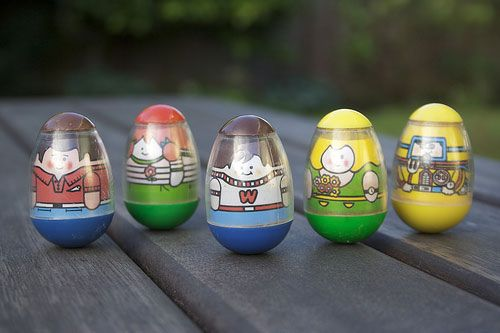
\includegraphics[width=0.6\textwidth,keepaspectratio]{./S01/img/13/weebles-toy.jpg}
    };
    \draw [white, rounded corners=\ClipSep, line width=\ClipSep]
    (current bounding box.north west) --
    (current bounding box.north east) --
    (current bounding box.south east) --
    (current bounding box.south west) -- cycle
    ;
    \end{tikzpicture}
    \caption{Weebles - Brinquedo\label{fig:weebles-brinquedo}}
\end{figure}

\hypertarget{kerplunk}{%
\section{KerPlunk}\label{kerplunk}}

\begin{figure}[!ht]
  \begin{adjustwidth}{-\oddsidemargin-1in}{-\rightmargin}
    \centering
    
\includegraphics[trim={0 9cm 0 1cm,}, clip, width=\paperwidth]{./S01/img/13/ker-plunk.png}
    % \caption{KerPlunk\label{fig:ker-plunk}}
  \end{adjustwidth}
\end{figure}

\begin{tcolorbox}[enhanced,center upper,
    drop fuzzy shadow southeast, boxrule=0.3pt,
    lower separated=false,
    colframe=black!30!dialogoBorder,colback=white]
\begin{minipage}[c]{0.16\linewidth}
  \raisebox{\dimexpr-\height+\ht\strutbox\relax}{
    \centering 
\includegraphics[width=1.4cm]{./assets/img/chandler.png}
  }
   & \centering \scriptsize{Chandler}
\end{minipage}
\hfill
\begin{minipage}[c]{0.8\linewidth}
  \textbf{- So who's up for a big game of Kerplunk?}\\
  - Quem quer jogar Kerplunk?
\end{minipage}
\end{tcolorbox}

Para quebrar o gelo após o encontro entre Ronnie e o Papai Joey,
Chandler sugere uma partida de \emph{KerPlunk} (1967), jogo de 2 a 4
competidores em que, em cada rodada, uma vareta deve ser retirada de um
tubo plástico, e em cima das varetas há bolinhas. O objetivo é derrubar
o menor número de bolinhas. No Brasil o jogo foi lançado pela
\emph{Estrela} com o nome \emph{Cai não cai}. \footnote{\sloppy KerPlunk - Ludopedia. \url{https://www.ludopedia.com.br/jogo/ker-plunk?v=}}
\footnote{\sloppy KerPlunk - YouTube (Inglês). \url{https://www.youtube.com/watch?v=Aslf72DPSR0}}

\begin{figure}
  \centering
  \begin{tikzpicture}
    \node [inner sep=0pt] at (0,0) {
      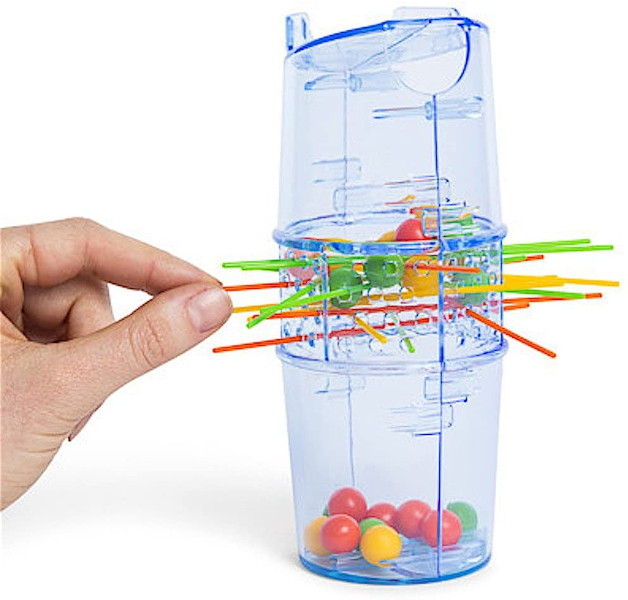
\includegraphics[width=0.6\textwidth,keepaspectratio]{./S01/img/13/ker-plunk-game.jpg}
    };
    \draw [white, rounded corners=\ClipSep, line width=\ClipSep]
    (current bounding box.north west) --
    (current bounding box.north east) --
    (current bounding box.south east) --
    (current bounding box.south west) -- cycle
    ;
    \end{tikzpicture}
    \caption{KerPlunk - Jogo\label{fig:ker-plunk-jogo}}
\end{figure}

\hypertarget{james-bond}{%
\section{James Bond}\label{james-bond}}

\begin{figure}[!ht]
  \begin{adjustwidth}{-\oddsidemargin-1in}{-\rightmargin}
    \centering
    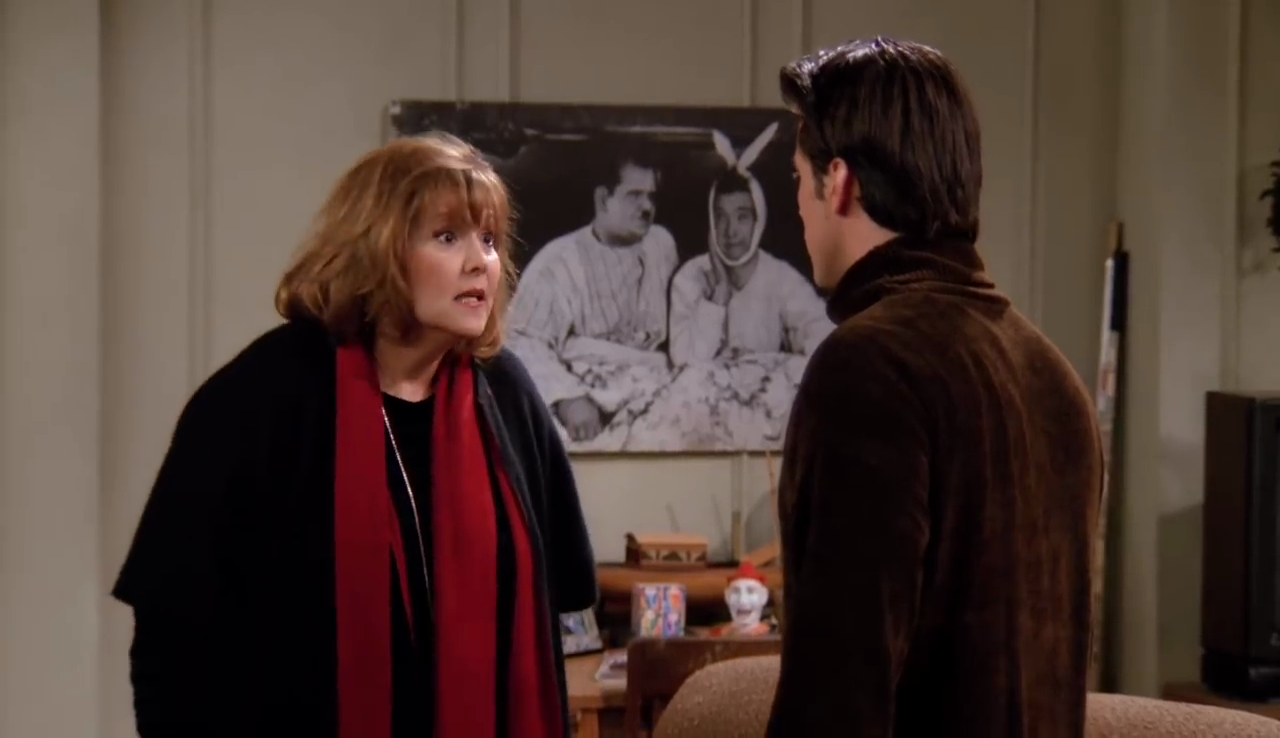
\includegraphics[trim={0 8cm 0 1cm,}, clip, width=\paperwidth]{./S01/img/13/james-bond.png}
    % \caption{James Bond\label{fig:james-bond}}
  \end{adjustwidth}
\end{figure}

\begin{tcolorbox}[enhanced,center upper,
    drop fuzzy shadow southeast, boxrule=0.3pt,
    lower separated=false, breakable,
    colframe=black!30!dialogoBorder,colback=white]
\begin{minipage}[c]{0.16\linewidth}
  \raisebox{\dimexpr-\height+\ht\strutbox\relax}{
    \centering 
\includegraphics[width=1.4cm]{./assets/img/joey.png}
  }
   & \centering \scriptsize{Joey}
\end{minipage}
\hfill
\begin{minipage}[c]{0.8\linewidth}
  \textbf{- Hold on. You knew?}\\
  - Espera aí. Você sabia?
\end{minipage}

\medskip
\begin{minipage}[c]{0.16\linewidth}
  \raisebox{\dimexpr-\height+\ht\strutbox\relax}{
    \centering 
\includegraphics[width=1.4cm]{./assets/img/gloria.png}
  }
   & \centering \scriptsize{Gloria}
\end{minipage}
\hfill
\begin{minipage}[c]{0.8\linewidth}
  \textbf{- Of course I knew. What do you think? Your father is no James Bond.}\\
  - Claro! O que achou? Seu pai não é James Bond.
\end{minipage}
\end{tcolorbox}

Gloria, mãe de Joey, menciona que Big Joey não é nenhum \emph{James
Bond} (1953), um agente secreto britânico fictício, protagonista da
franquia \emph{007}. Apareceu inicialmente no livro \emph{Casino
Royale}, para logo em seguida ser o mocinho de vários filmes.\footnote{\sloppy James Bond - Wikipédia. \url{https://pt.wikipedia.org/wiki/James_Bond}}

\hypertarget{sting}{%
\section{Sting}\label{sting}}

\begin{figure}[!ht]
  \begin{adjustwidth}{-\oddsidemargin-1in}{-\rightmargin}
    \centering
    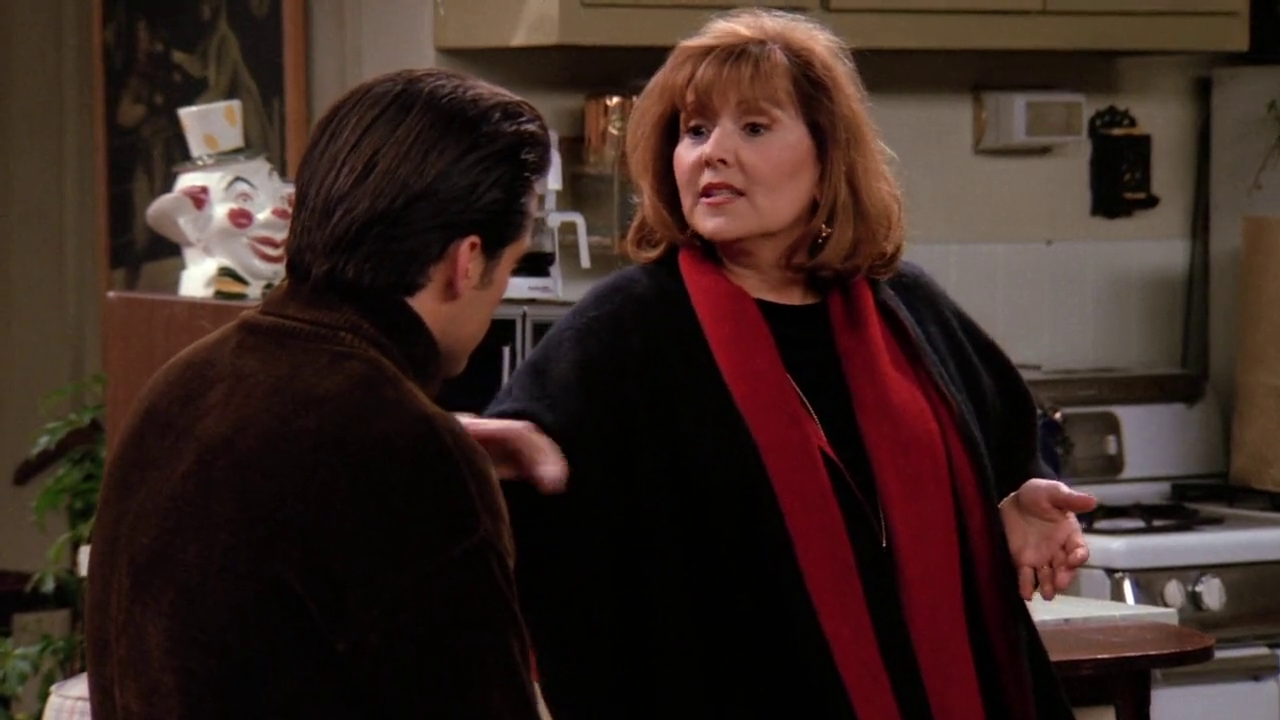
\includegraphics[trim={0 8cm 0 0cm,}, clip, width=\paperwidth]{./S01/img/13/sting.png}
    % \caption{Sting\label{fig:sting}}
  \end{adjustwidth}
\end{figure}

\begin{tcolorbox}[enhanced,center upper,
    drop fuzzy shadow southeast, boxrule=0.3pt,
    lower separated=false, breakable,
    colframe=black!30!dialogoBorder,colback=white]
\begin{minipage}[c]{0.16\linewidth}
  \raisebox{\dimexpr-\height+\ht\strutbox\relax}{
    \centering 
\includegraphics[width=1.4cm]{./assets/img/gloria.png}
  }
   & \centering \scriptsize{Gloria}
\end{minipage}
\hfill
\begin{minipage}[c]{0.8\linewidth}
  \textbf{- Look, honey, in an ideal world there'd be no her and your father would look like Sting.}\\
  - Ouça, em um mundo ideal ela não existiria e o seu pai se pareceria com o Sting.
\end{minipage}
\end{tcolorbox}

\saveparinfos
\noindent
\begin{minipage}[c]{0.5\textwidth}\useparinfo

Ponderando como seria se Big Joey fosse diferente, Gloria menciona
\emph{Sting} (1951), nome artístico de \emph{Gordon Matthew Thomas
Sumner}, conhecido por ser o vocalista da banda britânica \emph{The
Police} (Ver
\textbf{\textcolor{primarycolor}{S01E09 - Aquele em que o Oprimido Escapa}}).\footnote{\sloppy Sting - Site oficial. \url{https://www.sting.com/}}

\end{minipage}\hfill
\begin{minipage}[c]{0.5\textwidth}

\begin{figure}
  \centering
  \begin{tikzpicture}
    \node [inner sep=0pt] at (0,0) {
      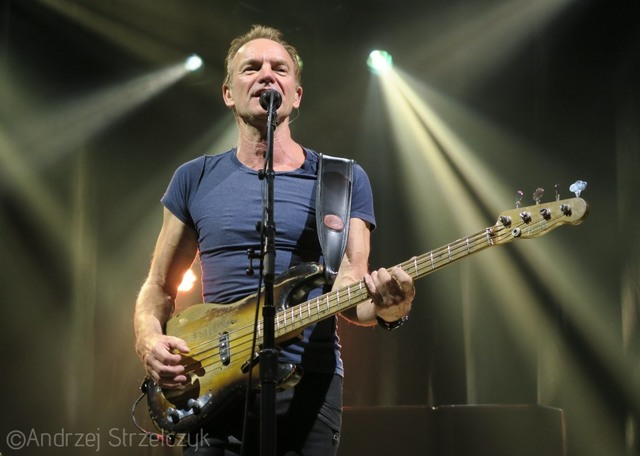
\includegraphics[width=0.8\textwidth,keepaspectratio]{./S01/img/13/sting-show.jpg}
    };
    \draw [white, rounded corners=\ClipSep, line width=\ClipSep]
    (current bounding box.north west) --
    (current bounding box.north east) --
    (current bounding box.south east) --
    (current bounding box.south west) -- cycle
    ;
    \end{tikzpicture}
    \caption{Sting - Show\label{fig:sting-show}}
\end{figure}

\end{minipage}

\hypertarget{waltons-mountain}{%
\section{Walton's Mountain}\label{waltons-mountain}}

\begin{figure}[!ht]
  \begin{adjustwidth}{-\oddsidemargin-1in}{-\rightmargin}
    \centering
    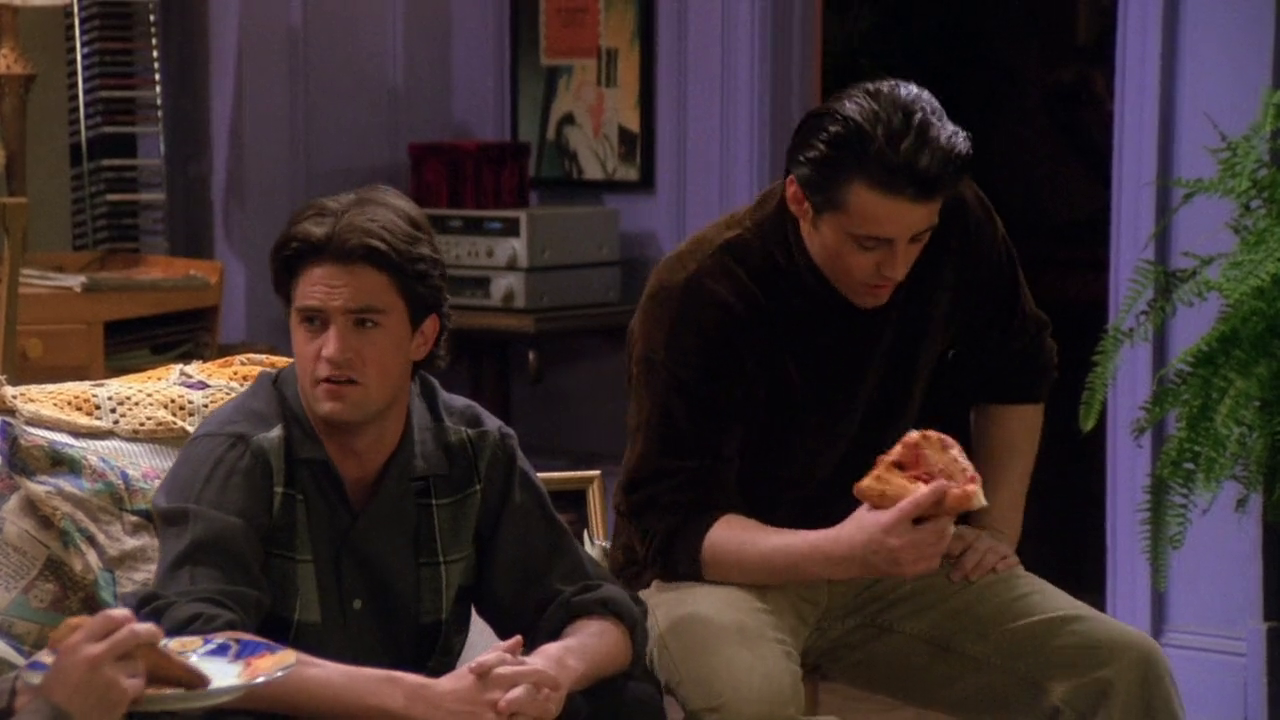
\includegraphics[trim={0 9cm 0 3cm,}, clip, width=\paperwidth]{./S01/img/13/walton-s-mountain.png}
    % \caption{Walton’s Mountain\label{fig:walton-s-mountain}}
  \end{adjustwidth}
\end{figure}

\begin{tcolorbox}[enhanced,center upper,
    drop fuzzy shadow southeast, boxrule=0.3pt,
    lower separated=false, breakable,
    colframe=black!30!dialogoBorder,colback=white]
\begin{minipage}[c]{0.16\linewidth}
  \raisebox{\dimexpr-\height+\ht\strutbox\relax}{
    \centering 
\includegraphics[width=1.4cm]{./assets/img/chandler.png}
  }
   & \centering \scriptsize{Chandler}
\end{minipage}
\hfill
\begin{minipage}[c]{0.8\linewidth}
  \textbf{- Things sure have changed here on Walton's mountain.}\\
  - Tudo mudou na montanha dos Walton.
\end{minipage}
\end{tcolorbox}

\saveparinfos
\noindent
\begin{minipage}[c]{0.5\textwidth}\useparinfo

Joey faz um resumo de tudo que aconteceu após a revelação da traição por
parte de seu pai. Chandler, sarcástico como sempre, cita \emph{Walton's
mountain}, local fictício onde se passa a história de \emph{The Waltons}
(1972), premiada série americana que tem como trama principal a história
de uma família que mora na zona rural da Virginia, na época entre a
\emph{Grande Depressão} (também conhecida como a \emph{Crise de 29}) e a
\emph{Segunda Guerra Mundial} (1939-1945).\footnote{\sloppy All about The Waltons. \url{http://www.allaboutthewaltons.com/}}

\end{minipage}\hfill
\begin{minipage}[c]{0.5\textwidth}

\begin{figure}
  \centering
  \begin{tikzpicture}
    \node [inner sep=0pt] at (0,0) {
      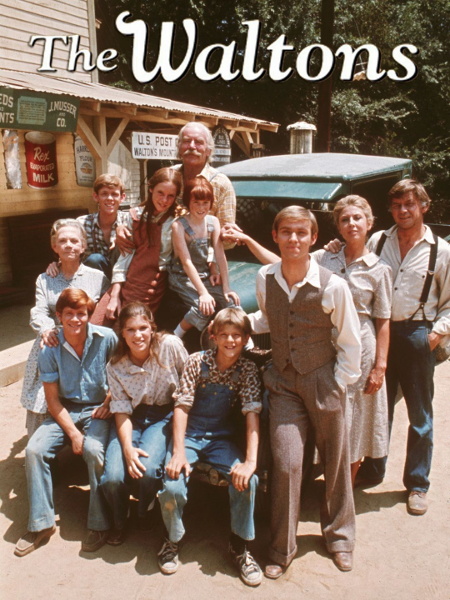
\includegraphics[width=0.8\textwidth,keepaspectratio]{./S01/img/13/the-waltons.jpg}
    };
    \draw [white, rounded corners=\ClipSep, line width=\ClipSep]
    (current bounding box.north west) --
    (current bounding box.north east) --
    (current bounding box.south east) --
    (current bounding box.south west) -- cycle
    ;
    \end{tikzpicture}
    \caption{The Waltons - Poster\label{fig:the-waltons-poster}}
\end{figure}

\end{minipage}
